\chaptercustom{2}{LỢI THẾ CỦA BIỂU DIỄN DPS SO VỚI SOCE}
\setcounter{section}{2}
\label{chap:dps_advantage}

\subsection{SoCE trực tiếp trong một chiều}
\label{subsec:ch2_1d_soce}

Chương 1 đã chỉ ra rằng nút thắt của mô phỏng kênh MIMO băng rộng nằm ở cách tính trực tiếp tổng các hàm mũ phức. Chương này chuyển từ nhận xét đó sang hai câu hỏi cụ thể: DPS giảm số chiều biểu diễn bằng cách nào, và trong điều kiện nào sự thay đổi cách biểu diễn có thể giảm khối lượng tính toán. Để tách phần cốt lõi khỏi mô hình bốn chiều, trước hết xét một tín hiệu SoCE một chiều gồm \(N\) mẫu:
\begin{equation}
h_m = \sum_{p=0}^{P-1}\eta_p e^{j2\pi \nu_p m},
\quad m=0,1,\ldots,N-1.
\label{eq:ch2_1d_soce}
\end{equation}
Trong \eqref{eq:ch2_1d_soce}, \(m\) là chỉ số mẫu; \(j\) là đơn vị ảo; \(\eta_p\) là trọng số phức của MPC thứ \(p\); còn \(\nu_p\) là tần số của MPC đó sau khi đã chuẩn hóa theo khoảng lấy mẫu. Tại mỗi giá trị \(m\), cần tính và cộng \(P\) số hạng. Do đó, khi tính đủ \(N\) mẫu, chi phí tính toán có bậc:
\begin{equation}
C_{\mathrm{SoCE},1\mathrm{D}}=\mathcal{O}(NP).
\label{eq:ch2_1d_soce_complexity}
\end{equation}

Ký hiệu \(\mathcal{O}(NP)\) cho biết chi phí tăng tỉ lệ theo tích của số mẫu và số MPC, nhưng không biểu diễn một số phép toán tuyệt đối. Khi mở rộng sang kênh MIMO băng rộng, một chỉ số \(m\) được thay bằng bốn chỉ số của thời gian, tần số, anten phát và anten thu. Số điểm phải tính khi đó bằng tích số mẫu trên bốn chiều. SoCE vẫn giữ ý nghĩa vật lý rõ ràng, nhưng phép tính trực tiếp chưa tận dụng việc tần số của các MPC chỉ nằm trong một miền hữu hạn.

\subsection{Tín hiệu giới hạn băng trên khối hữu hạn}
\label{subsec:ch2_bandlimited_block}

Giả sử các tần số chuẩn hóa trong \eqref{eq:ch2_1d_soce} nằm trong miền \([-W,W]\), với \(0<W<1/2\). Đại lượng \(W\) là nửa độ rộng miền băng; mốc \(1/2\) là biên Nyquist của tần số rời rạc đã chuẩn hóa. Khi đó, gom \(N\) mẫu thành véc-tơ
\begin{equation}
\mathbf{h}
= \begin{bmatrix}
h_0 & h_1 & \cdots & h_{N-1}
\end{bmatrix}^{T}
\label{eq:ch2_sample_vector}
\end{equation}
thì \(\mathbf{h}\) không phải là một véc-tơ tùy ý trong không gian \(\mathbb{C}^{N}\) gồm các véc-tơ phức có \(N\) phần tử. Mọi thành phần hàm mũ tạo nên \(\mathbf{h}\) đều có tần số thuộc \([-W,W]\), và tín hiệu chỉ được quan sát trên khối hữu hạn \(m=0,\ldots,N-1\). Hai ràng buộc này làm cho các phần tử của \(\mathbf{h}\) có quan hệ với nhau thay vì là \(N\) đại lượng độc lập hoàn toàn.

Số hệ số độc lập cần thiết để xấp xỉ tốt nhóm tín hiệu này được gọi là số bậc tự do hiệu dụng. Theo lý thuyết DPS, với miền đối xứng \([-W,W]\), số chiều thiết yếu xấp xỉ tích độ dài--băng thông \(2NW\) \cite{Slepian1978}. Đây là một giá trị xấp xỉ mô tả vị trí chuyển tiếp của các trị riêng, không phải quy tắc làm tròn duy nhất cho mọi mức sai số. Các chiều còn lại vẫn tồn tại về mặt đại số, nhưng thường đóng góp ít hơn vào biểu diễn tín hiệu giới hạn băng trên khối đang xét.

Đối với kênh MIMO băng rộng trong bài báo của Kaltenberger và cộng sự, lập luận này được áp dụng theo từng chiều: Doppler, trễ, góc khởi hành và góc tới \cite{Kaltenberger2007}. Khi miền giới hạn băng có dạng tích Descartes, không gian con đa chiều có thể xây dựng từ các không gian con DPS một chiều.

\subsection{Cơ sở DPS một chiều}
\label{subsec:ch2_1d_dps}

DPS được xác định thông qua bài toán tìm các chuỗi có năng lượng phổ tập trung nhiều nhất trong miền \([-W,W]\) khi chỉ xét \(N\) mẫu. Bài toán này được viết dưới dạng bài toán trị riêng. Với chiều dài \(N\) và nửa băng thông chuẩn hóa \(W\), mỗi véc-tơ DPS \(\mathbf{v}_d\) cùng trị riêng \(\lambda_d\) thỏa mãn:
\begin{equation}
\mathbf{C}_{N,W}\mathbf{v}_d = \lambda_d \mathbf{v}_d,
\quad d=0,1,\ldots,N-1,
\label{eq:ch2_dps_eigen}
\end{equation}
trong đó \(\mathbf{C}_{N,W}\) là ma trận tập trung băng có kích thước \(N\times N\), với phần tử:
\begin{equation}
\left[\mathbf{C}_{N,W}\right]_{m,n}
=
\begin{cases}
2W, & m=n,\\
\dfrac{\sin\!\left(2\pi W(m-n)\right)}{\pi(m-n)}, & m\ne n.
\end{cases}
\label{eq:ch2_dps_kernel}
\end{equation}
Các véc-tơ DPS có thể được chọn trực chuẩn và sắp xếp theo \(\lambda_0\geq\lambda_1\geq\cdots\geq\lambda_{N-1}\). Mỗi trị riêng nằm trong khoảng \([0,1]\) và biểu diễn tỉ lệ năng lượng phổ của véc-tơ tương ứng tập trung trong miền \([-W,W]\). Trị riêng gần \(1\) cho biết véc-tơ cơ sở phù hợp mạnh với miền băng cần biểu diễn; trị riêng gần \(0\) cho biết mức tập trung thấp. Vì vậy, thứ tự trị riêng cung cấp một tiêu chí để chọn các véc-tơ cơ sở đầu tiên.

Để minh họa trực tiếp tiêu chí này, Hình~\ref{fig:ch2_paper_figure4_dps_eigenvalues} trình bày kết quả tính toán bằng MATLAB với \(N=256\) và \(N\nu_{D,\max}=2\). Bộ tham số và cách xác định số chiều thiết yếu được lựa chọn dựa trên ví dụ trị riêng DPS của Kaltenberger và cộng sự \cite{Kaltenberger2007}. Trục ngang là chỉ số \(d\) của véc-tơ DPS, còn trục đứng là trị riêng \(\lambda_d\) trên thang logarit. Với cấu hình này, số chiều thiết yếu là \(D'=\lceil 2N\nu_{D,\max}\rceil+1=5\).

\begin{figure}[H]
    \centering
    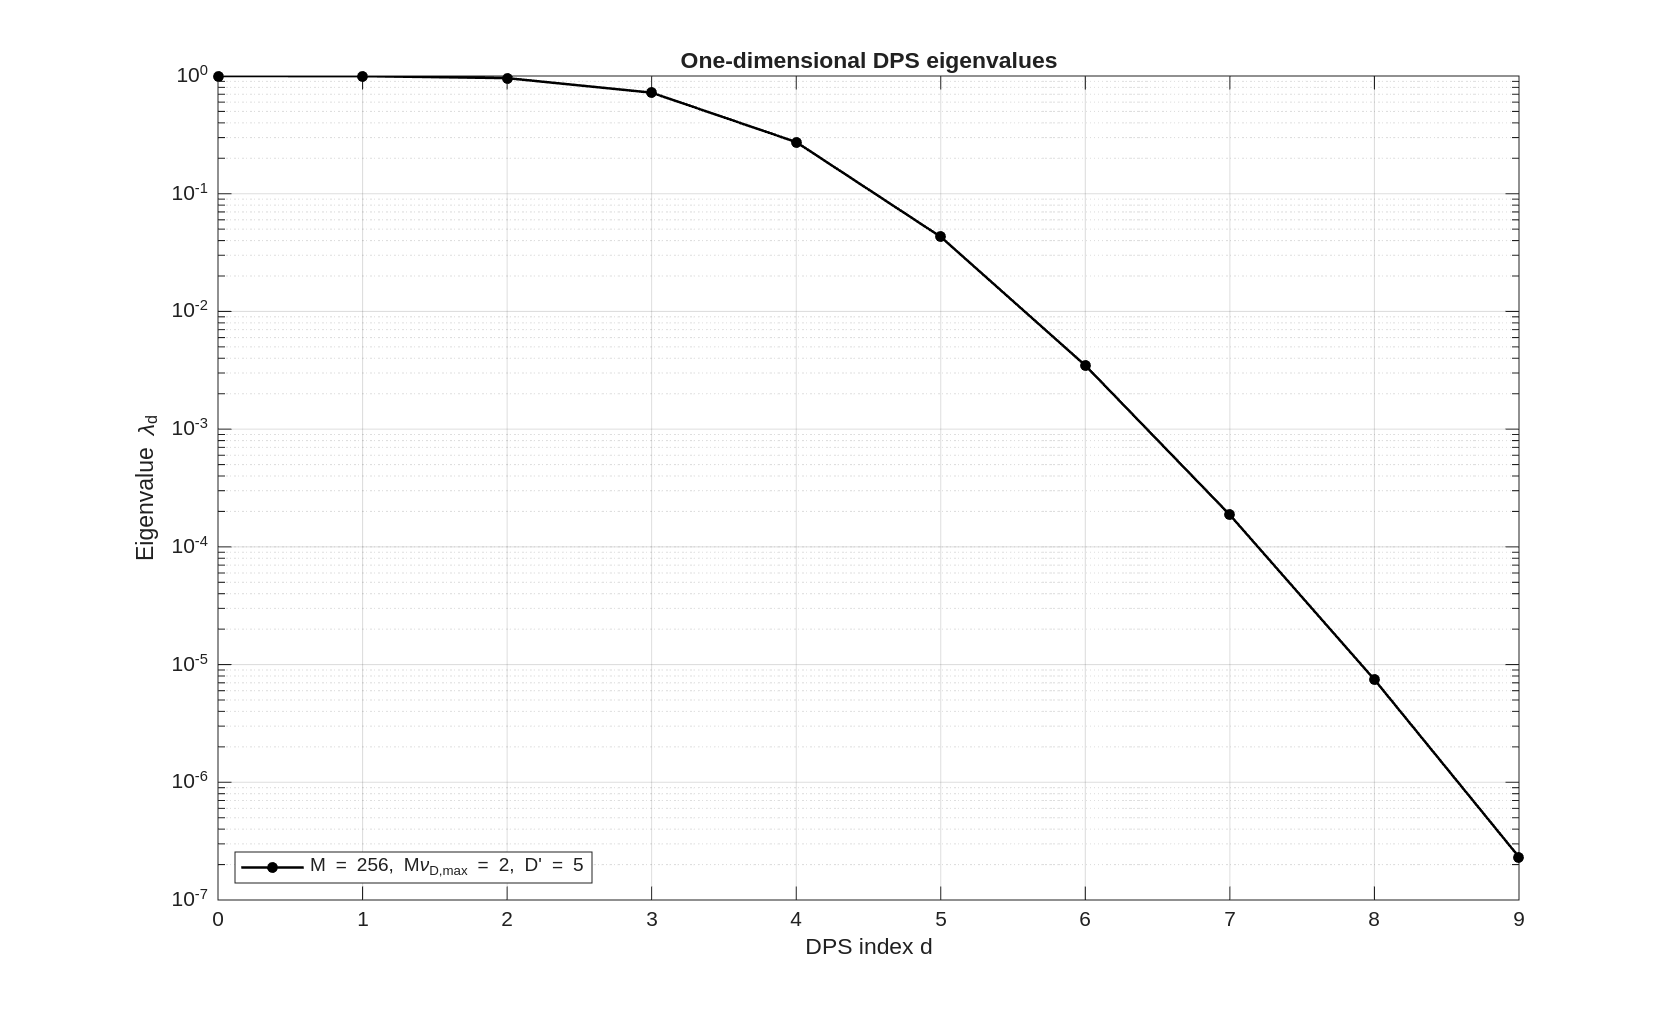
\includegraphics[width=0.9\textwidth]{results/figures/paper_figure4_dps_eigenvalues.png}
    \caption{Mười trị riêng đầu tiên của chuỗi DPS một chiều với \(N=256\) và \(N\nu_{D,\max}=2\)}
    \label{fig:ch2_paper_figure4_dps_eigenvalues}
\end{figure}

Hình~\ref{fig:ch2_paper_figure4_dps_eigenvalues} cho thấy các trị riêng đầu có giá trị lớn, sau đó giảm nhanh qua vùng chuyển tiếp quanh \(d=4\)--\(5\). Cụ thể, \(\lambda_0\approx0{,}99994\), trong khi \(\lambda_5\approx4{,}30\times10^{-2}\) và \(\lambda_9\approx2{,}32\times10^{-7}\). Do đó, các véc-tơ DPS có chỉ số lớn đóng góp ngày càng ít vào việc biểu diễn tín hiệu nằm trong băng Doppler mục tiêu. Đây là cơ sở để thay một véc-tơ kênh có \(256\) mẫu bằng một số lượng nhỏ hơn nhiều hệ số DPS; trong ví dụ của bài báo, khoảng năm chiều đầu tạo thành phần không gian con thiết yếu.

Tuy nhiên, \(D'=5\) chỉ mô tả vị trí chuyển tiếp của phổ trị riêng trong cấu hình cụ thể này, không phải số chiều cố định cho mọi kênh. Khi yêu cầu sai số nghiêm ngặt, có thể giữ thêm một số véc-tơ sau \(D'\). Ngược lại, nếu băng chuẩn hóa rộng hơn hoặc độ dài khối thay đổi, số chiều thiết yếu cũng thay đổi theo tích độ dài--băng thông. Vì vậy, kết luận cần rút ra từ hình là \(D\) có thể nhỏ hơn đáng kể \(N\) khi kênh bị giới hạn trong một miền Doppler hẹp, chứ không phải mọi kênh dài \(256\) mẫu đều luôn chỉ cần đúng năm véc-tơ DPS.

Nếu chọn \(D\) véc-tơ DPS đầu tiên và đặt:
\begin{equation}
\mathbf{V}
=
\begin{bmatrix}
\mathbf{v}_0 & \mathbf{v}_1 & \cdots & \mathbf{v}_{D-1}
\end{bmatrix},
\label{eq:ch2_dps_basis}
\end{equation}
thì \(\mathbf{V}\in\mathbb{C}^{N\times D}\) là ma trận cơ sở của một không gian con \(D\) chiều. Giữ nhiều véc-tơ hơn thường làm giảm phần năng lượng bị loại bỏ, nhưng đồng thời làm tăng số hệ số và chi phí tái tạo. Vì vậy, lựa chọn \(D\) thể hiện sự đánh đổi giữa độ phức tạp và sai số cắt không gian con.

\subsection{Biểu diễn không gian con DPS}
\label{subsec:ch2_dps_subspace}

Sau khi có ma trận cơ sở \(\mathbf{V}\), véc-tơ kênh được xấp xỉ dưới dạng tổ hợp tuyến tính của \(D\) cột trong ma trận này:
\begin{equation}
\hat{\mathbf{h}}^{D}=\mathbf{V}\boldsymbol{\alpha},
\label{eq:ch2_dps_reconstruction}
\end{equation}
trong đó dấu mũ trên \(\hat{\mathbf{h}}^{D}\) cho biết đây là véc-tơ tái tạo bằng \(D\) cơ sở, còn \(\boldsymbol{\alpha}\in\mathbb{C}^{D}\) chứa trọng số của từng cơ sở. Nếu \(\mathbf{V}\) trực chuẩn, hệ số chiếu chính xác của toàn bộ véc-tơ kênh được tính bằng:
\begin{equation}
\boldsymbol{\alpha}_{\mathrm{exact}}
= \mathbf{V}^{H}\mathbf{h}.
\label{eq:ch2_exact_projection}
\end{equation}
trong đó ký hiệu \((\cdot)^H\) là phép chuyển vị liên hợp. Công thức \eqref{eq:ch2_exact_projection} có ý nghĩa kiểm chứng rõ ràng: nếu tái tạo từ \(\boldsymbol{\alpha}_{\mathrm{exact}}\) cho sai số nhỏ, các \(D\) véc-tơ đã chọn giữ được phần quan trọng của khối kênh.

Có hai cách tương đương để thực hiện phép chiếu chính xác. Cách thứ nhất tạo toàn bộ \(\mathbf{h}\) bằng SoCE rồi áp dụng \eqref{eq:ch2_exact_projection}; cách này phù hợp để diễn giải nhưng vẫn phải tính đủ kênh tham chiếu. Cách thứ hai khai thác tính tuyến tính của phép chiếu: chiếu riêng véc-tơ hàm mũ của từng MPC lên \(\mathbf{V}\), nhân với \(\eta_p\), rồi cộng các hệ số. Mã mô phỏng dùng cách thứ hai và tiếp tục tách phép chiếu theo từng chiều. Phép chiếu vẫn là chính xác đối với cơ sở đã chọn, nhưng chi phí còn phụ thuộc vào tích giữa độ dài tín hiệu và số chiều cơ sở.

Để giảm tiếp chi phí tính các tích vô hướng này, bài báo Kaltenberger và cộng sự sử dụng công thức hàm sóng DPS nhằm xấp xỉ hệ số trực tiếp từ tần số của từng MPC \cite{Kaltenberger2007}. Trong đồ án, cách tính đó được gọi là DPS xấp xỉ. Như vậy, cần phân biệt sai số cắt do chỉ giữ \(D\) cơ sở với sai số bổ sung do dùng công thức xấp xỉ hệ số.

\subsection{So sánh cơ chế tính toán giữa SoCE và DPS}
\label{subsec:ch2_soce_dps_compare}

Sự khác nhau chính giữa SoCE và DPS nằm ở cách tổ chức phép tính. Với SoCE trực tiếp, giá trị kênh tại mỗi mẫu được tạo bằng cách cộng đóng góp của toàn bộ \(P\) MPC:
\begin{equation}
h_m
=\sum_{p=0}^{P-1}\eta_p e^{j2\pi\nu_p m}.
\label{eq:ch2_soce_samplewise}
\end{equation}
Cách tính này bám sát mô hình vật lý nhưng chi phí tăng theo cả số mẫu và số MPC. Ngược lại, với DPS, khối mẫu được biểu diễn thông qua các hệ số trong không gian con:
\begin{equation}
\hat{h}_m^{D}
= \sum_{d=0}^{D-1}\alpha_d v_d[m].
\label{eq:ch2_dps_samplewise}
\end{equation}
Khi \(D<N\), biểu diễn \eqref{eq:ch2_dps_samplewise} dùng ít hệ số hơn số mẫu ban đầu. Tuy nhiên, điều này chưa tự động bảo đảm tổng chi phí nhỏ hơn, vì vẫn phải tính hệ số và tái tạo \(N\) mẫu khi cần toàn bộ khối kênh. Lợi thế chỉ xuất hiện khi \(D\) đủ nhỏ và hai bước này được tổ chức hiệu quả.

Với tín hiệu giới hạn trong miền tần số chuẩn hóa \([-W,W]\) và chỉ xét trên \(N\) mẫu, lý thuyết DPS cho thấy số trị riêng lớn của bài toán \eqref{eq:ch2_dps_eigen} xấp xỉ bằng tích thời gian--băng thông \(2NW\) \cite{Slepian1978}. Do đó, số chiều DPS thiết yếu thường được chọn theo dạng:
\begin{equation}
D \approx 2NW + \Delta_D,
\label{eq:ch2_essential_dimension}
\end{equation}
trong đó \(\Delta_D\) là số chiều dự phòng được cộng thêm để giảm sai số cắt; giá trị cuối cùng của \(D\) phải là số nguyên. Khi \(W\) hẹp hơn đáng kể so với toàn miền tần số chuẩn hóa, \(2NW\) có thể nhỏ hơn nhiều so với \(N\). Khi đó, việc dùng các véc-tơ DPS đầu tiên có cơ sở từ cấu trúc giới hạn băng, thay vì chỉ là lựa chọn tùy ý. Trong mô phỏng của đồ án, số chiều dự phòng được chọn theo một quy tắc cố định và sẽ được nêu ở Chương 3.

Lập luận trên phù hợp với bài báo của Kaltenberger và cộng sự, trong đó kênh GCM sau rời rạc hóa được xem là tín hiệu giới hạn băng theo từng chiều và được chiếu lên không gian con DPS có số chiều hữu hạn \cite{Kaltenberger2007}. Như vậy, lợi thế của DPS không đến từ việc loại bỏ MPC khỏi mô hình, mà đến từ việc các tổ hợp SoCE có cùng miền giới hạn băng có thể được mô tả trong một không gian con chung. Nói cách khác, DPS chuyển bài toán từ tính từng tia truyền tại từng mẫu sang biểu diễn khối kênh bằng các hệ số không gian con.

Trong trường hợp nhiều chiều, khối mẫu được lưu dưới dạng tensor, tức mảng có nhiều hơn hai chiều. Giả sử tensor có kích thước \(N_1\times N_2\times\cdots\times N_L\), còn số véc-tơ DPS được giữ lại trên từng chiều là \(D_1,D_2,\ldots,D_L\). Khi đó, tổng số hệ số của biểu diễn tensor là:
\begin{equation}
D_{\mathrm{total}}=\prod_{\ell=1}^{L}D_\ell.
\label{eq:ch2_dps_total_dimension}
\end{equation}
Nếu chiều thứ \(\ell\) có nửa băng thông chuẩn hóa \(W_\ell\), lập luận thời gian--băng thông cho phép xấp xỉ:
\begin{equation}
D_{\mathrm{total}}
\approx
\prod_{\ell=1}^{L}\left(2N_\ell W_\ell+\Delta_{D_\ell}\right).
\label{eq:ch2_dps_total_dimension_approx}
\end{equation}
So sánh \eqref{eq:ch2_dps_total_dimension_approx} với tổng số mẫu \(\prod_{\ell=1}^{L}N_\ell\) cho thấy lợi thế về số chiều xuất hiện khi các miền băng \(W_\ell\) đủ hẹp để \(D_\ell<N_\ell\), đặc biệt khi điều kiện này đồng thời xảy ra trên nhiều chiều. Mức giảm thực tế còn phụ thuộc vào kích thước khối mẫu và sai số cắt không gian con được chấp nhận.

\subsection{Đối chứng triển khai cho biểu diễn DPS}
\label{subsec:ch2_alternative_baselines}

SoCE trực tiếp là tham chiếu tự nhiên vì bám sát các tham số vật lý của từng MPC. Tuy nhiên, nếu chỉ so sánh DPS với một cách cài đặt SoCE chưa tối ưu, phần giảm thời gian quan sát được có thể đến từ cách tính hàm mũ thay vì từ việc giảm số chiều. Vì vậy, SoCE cập nhật pha đệ quy được dùng như một đối chứng triển khai: phương pháp này giữ nguyên tập MPC và mô hình vật lý, nhưng thay cách tạo các thừa số pha. Đối chứng này giúp đánh giá liệu lợi thế của DPS còn được duy trì khi SoCE đã được tối ưu ở mức tạo pha.

\subsubsection{SoCE cập nhật pha đệ quy}
\label{subsubsec:ch2_recursive_soce}

Đặt \(z_p[m]=e^{j2\pi\nu_p m}\) và hệ số quay pha \(\rho_p=e^{j2\pi\nu_p}\). Các mẫu liên tiếp của MPC thứ \(p\) thỏa mãn:
\begin{equation}
z_p[0]=1,
\qquad
z_p[m+1]=\rho_p z_p[m].
\label{eq:ch2_recursive_phasor}
\end{equation}
Sau khi tính \(\rho_p\) một lần, các mẫu tiếp theo được tạo bằng phép nhân phức thay vì gọi lại hàm mũ. Giá trị kênh vẫn được cộng theo
\begin{equation}
h_m=\sum_{p=0}^{P-1}\eta_p z_p[m].
\label{eq:ch2_recursive_soce}
\end{equation}
Trong số học chính xác, \eqref{eq:ch2_recursive_soce} tương đương với SoCE trực tiếp trong \eqref{eq:ch2_1d_soce}; phương pháp không cắt bớt MPC và không lượng tử hóa tần số. Đối với lưới bốn chiều, quan hệ đệ quy có thể được áp dụng riêng cho các thừa số pha theo thời gian, tần số, anten phát và anten thu. Bậc độ phức tạp vẫn là \(\mathcal{O}(PN_{\mathrm{s}})\), nhưng số lần đánh giá hàm mũ được chuyển chủ yếu sang bước khởi tạo. Đổi lại, phép nhân lặp trong số học dấu phẩy động có thể tích lũy sai số biên độ và pha trên khối rất dài. Do đó, đây là đối chứng cần thiết để đánh giá liệu lợi thế của DPS còn được duy trì khi SoCE đã được tối ưu ở mức tạo pha.

\subsection{So sánh độ phức tạp và số phép tính}
\label{subsec:ch2_operation_count}

Phần trên so sánh số chiều biểu diễn. Để chuyển sang chi phí tính toán, cần tách ba nhóm phép toán của DPS: tính các hệ số một chiều, ghép chúng thành tensor hệ số và tái tạo khối mẫu. Trước hết, ký hiệu:
\begin{equation}
N_{\mathrm{s}}
=MQN_{\mathrm{Tx}}N_{\mathrm{Rx}}
\label{eq:ch2_total_samples}
\end{equation}
là tổng số mẫu của một khối kênh MIMO băng rộng. Với SoCE trực tiếp, mỗi mẫu cần cộng đóng góp của \(P\) MPC. Vì vậy, số hạng MPC--mẫu cần xử lý là:
\begin{equation}
N_{\mathrm{SoCE}}
=PN_{\mathrm{s}}
=PMQN_{\mathrm{Tx}}N_{\mathrm{Rx}}.
\label{eq:ch2_soce_operation_count}
\end{equation}
Nếu các hàm mũ một chiều đã được tạo trước, mỗi số hạng trong \eqref{eq:ch2_soce_operation_count} vẫn cần các phép nhân phức để ghép bốn chiều và cộng vào kênh tổng. Do đó, bậc độ phức tạp của SoCE trực tiếp vẫn là \(\mathcal{O}(PN_{\mathrm{s}})\).

Với biểu diễn DPS bốn chiều, ký hiệu \(D_t\), \(D_f\), \(D_{\mathrm{Tx}}\) và \(D_{\mathrm{Rx}}\) lần lượt là số véc-tơ DPS giữ lại trên các chiều thời gian, tần số, không gian phát và không gian thu. Số hệ số cần lưu trong tensor là \(D_{\mathrm{total}}=D_tD_fD_{\mathrm{Tx}}D_{\mathrm{Rx}}\). Nếu hệ số của từng MPC được tính bằng phép chiếu chính xác một chiều, chi phí tạo bốn véc-tơ hệ số một chiều có bậc:
\begin{equation}
C_{\gamma,\mathrm{exact}}
=
\mathcal{O}\!\left(
P(MD_t+QD_f+N_{\mathrm{Tx}}D_{\mathrm{Tx}}+N_{\mathrm{Rx}}D_{\mathrm{Rx}})
\right).
\label{eq:ch2_exact_gamma_complexity}
\end{equation}
Sau đó, việc cộng đóng góp của từng MPC vào tensor hệ số cần thêm:
\begin{equation}
C_{\alpha,\mathrm{4D}}
=
\mathcal{O}\!\left(PD_tD_fD_{\mathrm{Tx}}D_{\mathrm{Rx}}\right).
\label{eq:ch2_alpha_4d_complexity}
\end{equation}
Tiếp theo, tensor hệ số được nhân lần lượt với ma trận cơ sở trên từng chiều; thao tác trên một chiều của tensor thường được gọi là phép nhân theo mode. Chi phí tái tạo có bậc:
\begin{equation}
\begin{aligned}
C_{\mathrm{rec},\mathrm{4D}}
=\mathcal{O}\big(
&MD_tD_fD_{\mathrm{Tx}}D_{\mathrm{Rx}}
+MQD_fD_{\mathrm{Tx}}D_{\mathrm{Rx}}\\
&+MQN_{\mathrm{Tx}}D_{\mathrm{Tx}}D_{\mathrm{Rx}}
+MQN_{\mathrm{Tx}}N_{\mathrm{Rx}}D_{\mathrm{Rx}}
\big).
\end{aligned}
\label{eq:ch2_4d_reconstruction_complexity}
\end{equation}
Các biểu thức \eqref{eq:ch2_exact_gamma_complexity}--\eqref{eq:ch2_4d_reconstruction_complexity} cho thấy DPS tổ chức lại phép tính: phần phụ thuộc vào số MPC được chuyển chủ yếu sang việc tạo tensor hệ số có kích thước \(D_{\mathrm{total}}\), sau đó kênh được tái tạo từ tensor này. Khi các \(D\) đủ nhỏ so với số mẫu tương ứng, tổng số phép tính có khả năng giảm; ngược lại, nếu các \(D\) tiến gần kích thước khối, chi phí tái tạo có thể làm mất lợi thế.

Đối với nhánh DPS xấp xỉ 4D, hệ số một chiều được tính trực tiếp từ tần số chuẩn hóa của MPC bằng công thức hàm sóng DPS, thay vì chiếu chính xác lên toàn bộ véc-tơ hàm mũ. Nếu bỏ qua chi phí tiền xử lý cơ sở độ phân giải cao, phần hệ số một chiều có bậc:
\begin{equation}
C_{\gamma,\mathrm{approx}}
=
\mathcal{O}\!\left(P(D_t+D_f+D_{\mathrm{Tx}}+D_{\mathrm{Rx}})\right).
\label{eq:ch2_approx_gamma_complexity}
\end{equation}
Phương pháp kết hợp (hybrid) chỉ dùng DPS ở hai chiều thời gian và tần số, còn đáp ứng theo từng cặp anten được giữ trực tiếp. Khi đó tensor hệ số có kích thước \(D_tD_fN_{\mathrm{Tx}}N_{\mathrm{Rx}}\), và chi phí tái tạo chính là:
\begin{equation}
C_{\mathrm{rec},\mathrm{hybrid}}
=
\mathcal{O}\!\left(
MD_tD_fN_{\mathrm{Tx}}N_{\mathrm{Rx}}
+MQD_fN_{\mathrm{Tx}}N_{\mathrm{Rx}}
\right).
\label{eq:ch2_hybrid_reconstruction_complexity}
\end{equation}

Để đặt các biểu thức trên trong cùng một khung so sánh, Bảng~\ref{tab:ch2_complexity_comparison} tóm tắt bậc độ phức tạp và nguồn sai số của các phương pháp.

\begin{table}[H]
    \centering
    \small
    \caption{So sánh lý thuyết giữa SoCE và các nhánh DPS}
    \label{tab:ch2_complexity_comparison}
    \begin{tabularx}{\textwidth}{>{\raggedright\arraybackslash}p{0.17\textwidth} >{\raggedright\arraybackslash}p{0.25\textwidth} >{\raggedright\arraybackslash}p{0.24\textwidth} >{\raggedright\arraybackslash}X}
        \toprule
        Phương pháp & Phần phụ thuộc MPC hoặc hệ số & Tái tạo khối kênh & Đặc điểm sai số và điều kiện áp dụng \\
        \midrule
        SoCE trực tiếp
        & Không có bước hệ số riêng
        & \(\mathcal{O}(PN_{\mathrm{s}})\)
        & Tham chiếu theo mô hình MPC; chi phí tăng theo cả \(P\) và số mẫu. \\
        SoCE đệ quy
        & Khởi tạo các hệ số quay pha theo từng MPC và từng chiều
        & \(\mathcal{O}(PN_{\mathrm{s}})\)
        & Tương đương SoCE về mặt toán học; giảm số lần gọi hàm mũ nhưng có thể tích lũy sai số làm tròn. \\
        DPS chính xác 4D
        & \(C_{\gamma,\mathrm{exact}}+\mathcal{O}(PD_{\mathrm{total}})\)
        & \(C_{\mathrm{rec},\mathrm{4D}}\)
        & Hệ số chiếu chính xác trên cơ sở giữ lại; còn sai số cắt không gian con. \\
        DPS xấp xỉ 4D
        & \(\mathcal{O}(P\sum_iD_i)+\mathcal{O}(PD_{\mathrm{total}})\)
        & \(C_{\mathrm{rec},\mathrm{4D}}\)
        & Có sai số cắt và sai số xấp xỉ hệ số; cần bộ nhớ cho cơ sở độ phân giải cao. \\
        Hybrid DPS
        & Tạo hệ số DPS theo thời gian--tần số và giữ trực tiếp hai chiều không gian
        & \(C_{\mathrm{rec},\mathrm{hybrid}}\)
        & Tránh xấp xỉ DPS theo không gian; phù hợp khi số anten nhỏ so với số mẫu thời gian--tần số. \\
        \bottomrule
    \end{tabularx}
\end{table}

Bảng~\ref{tab:ch2_complexity_comparison} cho thấy SoCE đệ quy không thay đổi bậc \(\mathcal{O}(PN_{\mathrm{s}})\); lợi ích của nó nằm ở hằng số thực thi. DPS tổ chức lại phép tính thông qua không gian con, nên lợi thế của nó xuất hiện khi \(D_i\ll N_i\) trên các chiều có miền băng hẹp. Vì vậy, một đánh giá thực nghiệm công bằng phải dùng cùng tập MPC, cùng khối đầu ra và tính cả thời gian tiền xử lý, tạo hệ số lẫn tái tạo.

Bảng~\ref{tab:ch2_operation_estimate} minh họa các đại lượng trên với cấu hình hiện tại: \(M=256\), \(Q=64\), \(N_{\mathrm{Tx}}=N_{\mathrm{Rx}}=4\), \(P=80\), \(D_t=6\), \(D_f=9\) và \(D_{\mathrm{Tx}}=D_{\mathrm{Rx}}=4\). Các giá trị là ước lượng từ kích thước mảng và các biểu thức độ phức tạp, không phải số đếm chính xác mọi phép toán của MATLAB. Các số đo thời gian chạy được trình bày riêng ở Chương 4.

\begin{table}[H]
    \centering
    \small
    \caption{Ước lượng số phép xử lý chính với cấu hình mô phỏng hiện tại}
    \label{tab:ch2_operation_estimate}
    \begin{tabularx}{\textwidth}{l r >{\raggedright\arraybackslash}X}
        \toprule
        Đại lượng & Giá trị & Ý nghĩa \\
        \midrule
        \(N_{\mathrm{s}}=MQN_{\mathrm{Tx}}N_{\mathrm{Rx}}\) & \(262144\) & Số mẫu của một khối kênh 4D \\
        \(D_{\mathrm{total}}=D_tD_fD_{\mathrm{Tx}}D_{\mathrm{Rx}}\) & \(864\) & Số hệ số của biểu diễn DPS 4D \\
        \(N_{\mathrm{s}}/D_{\mathrm{total}}\) & \(\approx 303\) & Tỉ lệ giữa số mẫu kênh và số hệ số DPS 4D \\
        \(PN_{\mathrm{s}}\) & \(20971520\) & Số hạng MPC--mẫu trong SoCE trực tiếp \\
        \(4PN_{\mathrm{s}}\) & \(83886080\) & Ước lượng phép nhân phức để ghép bốn chiều nếu các hàm mũ một chiều đã có \\
        \(P(MD_t+QD_f+N_{\mathrm{Tx}}D_{\mathrm{Tx}}+N_{\mathrm{Rx}}D_{\mathrm{Rx}})\) & \(171520\) & Phép chiếu một chiều trong nhánh DPS chính xác \\
        \(PD_{\mathrm{total}}\) & \(69120\) & Cập nhật tensor hệ số DPS 4D theo từng MPC \\
        \(C_{\mathrm{rec},\mathrm{4D}}\) & \(4677632\) & Ước lượng phép nhân--cộng khi tái tạo DPS 4D \\
        \(C_{\mathrm{rec},\mathrm{hybrid}}\) & \(2580480\) & Ước lượng phép nhân--cộng khi tái tạo phương pháp hybrid \\
        \bottomrule
    \end{tabularx}
\end{table}

Từ Bảng~\ref{tab:ch2_operation_estimate}, số hệ số DPS 4D bằng \(864\), trong khi khối kênh chứa \(262144\) mẫu, tương ứng tỉ lệ xấp xỉ \(303\). Tỉ lệ này cho thấy khả năng nén về số hệ số, nhưng không đồng nghĩa thời gian chạy giảm đúng \(303\) lần vì vẫn có chi phí tạo cơ sở, tính hệ số và tái tạo. Trong cùng bảng, các ước lượng cho phép chiếu, cập nhật hệ số và tái tạo nhỏ hơn số hạng MPC--mẫu của SoCE trực tiếp trong cấu hình đang xét. Vì vậy, kết luận phù hợp là DPS có khả năng giảm độ phức tạp khi miền băng hẹp và \(D_{\mathrm{total}}\ll N_{\mathrm{s}}\), chứ không phải luôn có lợi trong mọi cấu hình.

\subsection{Ba mức tính hệ số trong đồ án}
\label{subsec:ch2_three_coefficients}

Để giữ thống nhất giữa lý thuyết và mô phỏng MATLAB, cần phân biệt ba nhánh theo cách tạo hệ số hoặc theo các chiều áp dụng DPS.

Thứ nhất, nhánh DPS chính xác tính tích vô hướng giữa véc-tơ hàm mũ của từng MPC và cơ sở DPS, sau đó ghép các hệ số một chiều thành tensor. Từ ``chính xác'' ở đây chỉ cách tính hệ số chiếu đối với cơ sở đã chọn; kênh tái tạo vẫn có thể có sai số vì cơ sở đã bị cắt còn \(D\) chiều. Nếu nhánh này có sai số nhỏ so với SoCE tham chiếu, số chiều DPS đang giữ là phù hợp với miền băng và khối mẫu đang xét.

Thứ hai, nhánh DPS xấp xỉ 4D thay các tích vô hướng chính xác bằng công thức hàm sóng DPS được đánh giá tại tần số chuẩn hóa của MPC. Công thức được áp dụng trên cả bốn chiều, nên sai số của nhánh này gồm cả sai số cắt không gian con và sai số xấp xỉ hệ số.

Thứ ba, phương pháp hybrid dùng hệ số DPS xấp xỉ cho hai chiều thời gian và tần số, trong khi phần không gian anten được tính bằng các hàm mũ trực tiếp. Với số anten nhỏ, số chiều không gian vốn đã thấp nên việc tiếp tục thay bằng cơ sở DPS có thể đem lại ít lợi ích hơn so với chi phí phát sinh. Nhánh hybrid vì vậy giữ khả năng giảm số chiều ở thời gian và tần số, đồng thời tránh xấp xỉ hệ số DPS trên hai chiều không gian.

\subsection{Đánh đổi khi sử dụng DPS}
\label{subsec:ch2_tradeoff}

DPS không làm cho mô phỏng kênh luôn đơn giản hơn trong mọi cấu hình. Lợi thế có khả năng xuất hiện khi miền tần số chuẩn hóa hẹp và số chiều thiết yếu nhỏ hơn đáng kể số mẫu ban đầu. Trong trường hợp đó, kênh được mô tả bằng ít hệ số hơn; với phép chiếu chính xác, sai số tái tạo chủ yếu đến từ phần năng lượng nằm ngoài không gian con đã chọn.

Ngược lại, nếu miền giới hạn băng rộng, tích \(2NW\) lớn hoặc số chiều dự phòng cao, \(D\) có thể tiến gần \(N\). Khi đó, lợi thế về số chiều giảm. Ngoài ra, cách tính hệ số xấp xỉ cần cơ sở trên lưới có độ phân giải cao để hạn chế sai số, làm phát sinh chi phí bộ nhớ và tiền xử lý. Vì vậy, việc sử dụng DPS phải được đánh giá đồng thời theo \(N\), \(W\), \(D\), số MPC, độ phân giải xấp xỉ và nhu cầu tái tạo toàn bộ khối kênh.

Trong phạm vi mô phỏng hiện tại, SoCE được dùng làm kênh tham chiếu; DPS chính xác dùng để đánh giá chất lượng không gian con; DPS xấp xỉ 4D và phương pháp hybrid dùng để khảo sát khả năng giảm độ phức tạp khi hệ số không được tính từ toàn bộ khối SoCE. Ngoài nhóm nhánh DPS này, SoCE đệ quy đóng vai trò đối chứng để kiểm tra ảnh hưởng của cách tạo pha.

\subsection{Kết luận chương}
\label{subsec:ch2_conclusion}

Chương này đã trả lời hai câu hỏi đầu chương. DPS giảm số chiều biểu diễn bằng cách dùng các véc-tơ cơ sở có mức tập trung năng lượng cao trong miền băng của kênh; số chiều thiết yếu được liên hệ với tích \(2NW\). So với việc tính từng MPC tại từng mẫu bằng SoCE, DPS tổ chức phép tính thành các bước tạo hệ số và tái tạo từ không gian con. SoCE đệ quy cho thấy việc tối ưu tạo pha có thể giảm hằng số thực thi nhưng không thay đổi bậc phụ thuộc \(PN_{\mathrm{s}}\). Vì vậy, lợi thế của DPS chỉ có khả năng xuất hiện khi số chiều giữ lại đủ nhỏ và chi phí tạo cơ sở, tính hệ số, tái tạo không làm mất phần tiết kiệm. Chương 3 tiếp tục cụ thể hóa các đại lượng này cho mô hình MIMO băng rộng bốn chiều và các nhánh mô phỏng MATLAB.

\cleardoublepage
